\chapter{Nemotron 3 Super Architecture}
\label{ch:arch}

\section{Overview}

\NS\ 120B-A12B~\cite{nvidia2026super} has 120.6 billion parameters in total
and 12.7 billion active per token. It scales up the hybrid Mamba--attention MoE
design of \NN~\cite{nvidia2025nano3} and is the first model in the family to
use \textbf{LatentMoE}, \textbf{Multi-Token Prediction (MTP)} for native
speculative decoding, and \textbf{NVFP4} pretraining
(Chapter~\ref{ch:training}). Table~\ref{tab:arch} lists its main dimensions.

\begin{table}[!htbp]
\centering
\small
\caption[Architectural dimensions of Nemotron 3 Super]{Architectural dimensions
of \NS\ (from~\cite{nvidia2026super}, Table~1)}
\label{tab:arch}
\begin{tabular}{@{}lr@{\hspace{2.5em}}lr@{}}
\toprule
\textbf{Configuration} & \textbf{Value} & \textbf{Configuration} & \textbf{Value} \\
\midrule
Total layers & 88 & Mamba heads / head dim. & 128 / 64 \\
Hidden dimension $d$ & 4096 & Mamba state dimension & 128 \\
Attention query heads & 32 & Experts per layer $N$ & 512 \\
Attention KV heads & 2 & Active experts (top-$k$) & 22 \\
Attention head dimension & 128 & Expert hidden dimension & 2688 \\
MTP layers (shared) & 2 & MoE latent size $\ell$ & 1024 \\
\bottomrule
\end{tabular}
\end{table}

\section{Hybrid Interleaved Layout}

Every sequence mixer---a Mamba-2 block or, occasionally, an attention
block---is followed by a LatentMoE layer (Figure~\ref{fig:layer-pattern}). Of
the 88 layers, 40 are Mamba-2, 40 are LatentMoE and only 8 are attention
layers, about 9\% of the stack, in line with the roughly 8\% found optimal by
Waleffe et al.~\cite{waleffe2024empirical}.

\begin{figure}[!htbp]
  \centering
  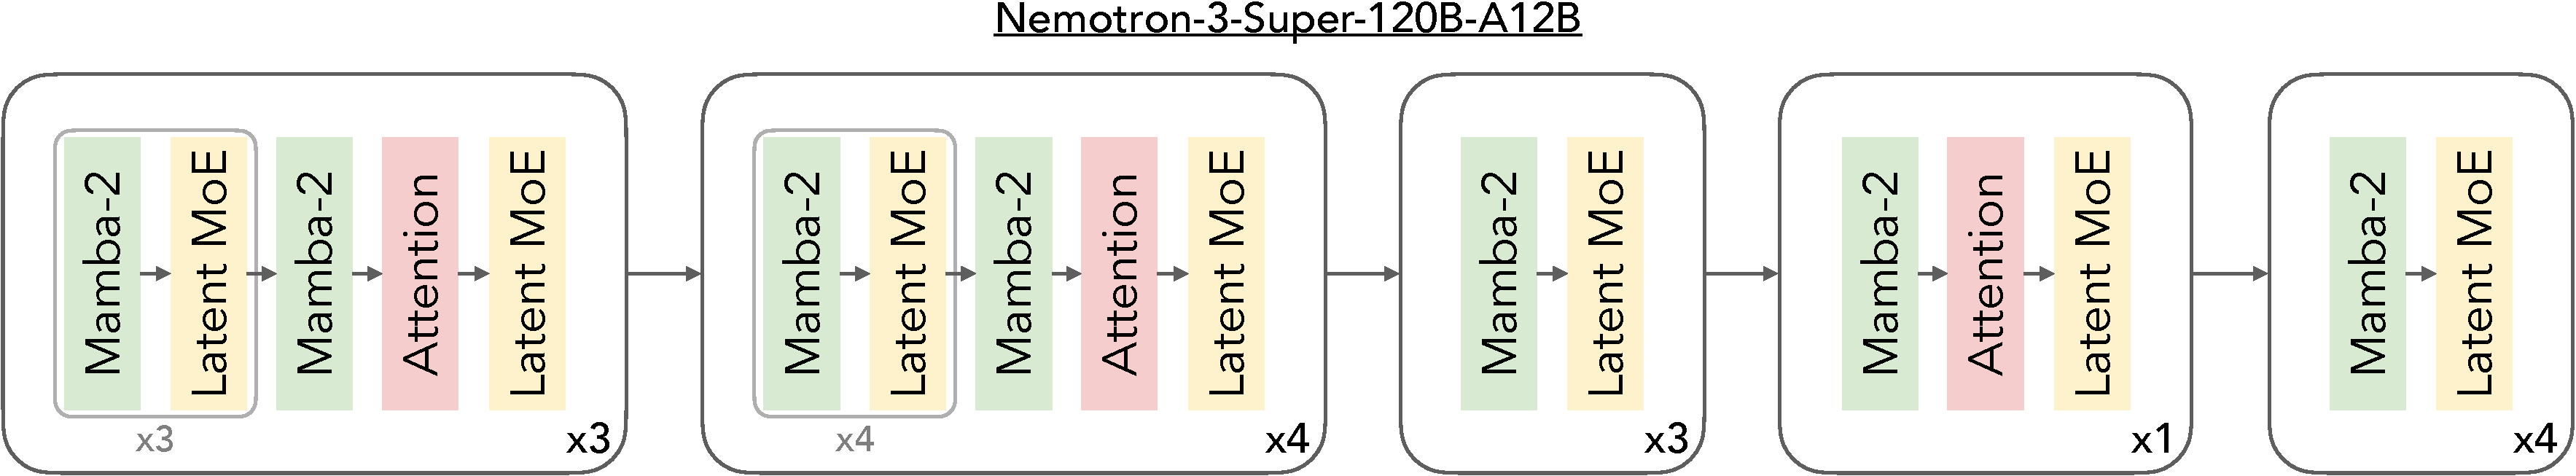
\includegraphics[width=\linewidth]{n3s-fig02-layer-pattern.pdf}
  \caption[Nemotron 3 Super layer pattern]{\NS\ layer pattern: Mamba-2 blocks
  paired with LatentMoE layers, with a few attention layers at intervals.
  \source{NVIDIA (2026)~\cite{nvidia2026super}, Fig.~2}}
  \label{fig:layer-pattern}
\end{figure}

Multiplying out the repeat counts in the pattern gives the layer budget in
Table~\ref{tab:layer-count}. Seven of the eight attention layers fall within
the first 71 layers, and the final eight layers contain none.

\begin{table}[!htbp]
\centering
\small
\caption[Layer budget of Nemotron 3 Super]{Layer budget of \NS, counted by the
author from the published layer pattern}
\label{tab:layer-count}
\begin{tabular}{@{}lcccc@{}}
\toprule
\textbf{Group in the pattern} & \textbf{Mamba-2} & \textbf{Attention} & \textbf{LatentMoE} & \textbf{Layers} \\
\midrule
$[\,(\text{M},\text{E})\times 3,\ \text{M},\ \text{A},\ \text{E}\,]\times 3$ & 12 & 3 & 12 & 27 \\
$[\,(\text{M},\text{E})\times 4,\ \text{M},\ \text{A},\ \text{E}\,]\times 4$ & 20 & 4 & 20 & 44 \\
$(\text{M},\text{E})\times 3$ & 3 & 0 & 3 & 6 \\
$(\text{M},\ \text{A},\ \text{E})\times 1$ & 1 & 1 & 1 & 3 \\
$(\text{M},\text{E})\times 4$ & 4 & 0 & 4 & 8 \\
\midrule
\textbf{Total} & \textbf{40} & \textbf{8} & \textbf{40} & \textbf{88} \\
\bottomrule
\multicolumn{5}{@{}l}{\footnotesize M = Mamba-2 block, A = attention block, E = LatentMoE layer.}
\end{tabular}
\end{table}

The layout is a division of labour. The Mamba-2 blocks do the heavy lifting in
linear time with a constant-size state. The few attention layers act as global
\emph{anchors} where every token can reach every other token, so information
that the Mamba state compressed away can still be retrieved exactly. The
attention layers use GQA with 32 query heads and only 2 KV heads; there are no
positional embeddings, and RMSNorm is used for normalisation.

The saving is large. By the author's estimate, 8 attention layers with 2 KV
heads of dimension 128 store $8 \times 2 \times 2 \times 128 = 4096$ numbers
per token, about 4\,GB at one million tokens in 8-bit precision; using
attention in place of all 40 Mamba blocks too would make it six times larger.
The 40 Mamba-2 states together hold about 42 million numbers---a few tens of
megabytes---regardless of context length.

\section{LatentMoE}

Each MoE layer has 512 experts, 22 of them active per token. LatentMoE~\cite{elango2026latentmoe}
starts from the observation that existing MoE designs are tuned for accuracy
per FLOP, whereas real deployments are limited by other things. NVIDIA's
analysis gives five principles~\cite{nvidia2026super}:
\begin{enumerate}
  \item In low-latency serving the cost is the \emph{memory bandwidth} to read
        expert weights of size $d \times m$, where $d$ is the hidden dimension
        and $m$ the expert's intermediate dimension.
  \item In distributed serving the cost is all-to-all \emph{routing} of tokens,
        whose volume scales as $d \times K$ for $K$ active experts.
  \item Quality depends on the non-linear budget $K \cdot m$, so $K$ and $m$
        should not be reduced.
  \item $d$ can be reduced only down to a task-dependent effective rank;
        below it, quality collapses.
  \item More experts $N$ and more active experts $K$ improve quality, because
        the number of expert combinations grows exponentially.
\end{enumerate}
Principles 1--3 single out $d$ as the quantity to shrink, principle 4 limits
how far, and principle 5 says how to spend the savings. Each token is projected from dimension $d$
into a smaller latent space of size $\ell$, the routed experts work there, and
the result is projected back (Figure~\ref{fig:latentmoe}):
\begin{equation}
  y = W_{\uparrow} \sum_{i \,\in\, \operatorname{TopK}(g(x),\,K')}
      g_i(x)\, E_i\bigl(W_{\downarrow}\,x\bigr) \;+\; E_{\text{shared}}(x).
  \label{eq:latentmoe}
\end{equation}
This cuts weight loads and routing traffic by $\alpha = d/\ell$, and the
saving is spent on $\alpha$ times more experts, improving quality at roughly
the same cost.

\begin{figure}[!htbp]
  \centering
  \begin{subfigure}[t]{0.42\linewidth}
    \centering
    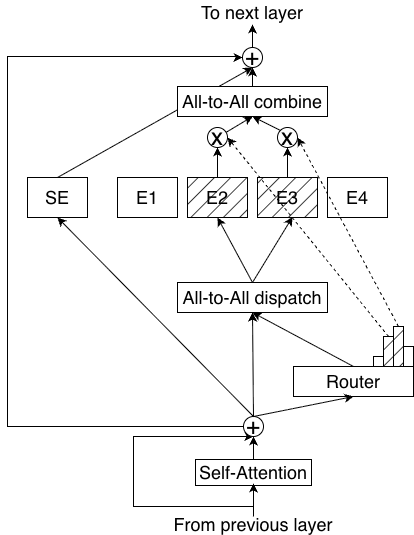
\includegraphics[width=\linewidth]{n3s-fig03a-standard-moe.png}
    \caption{Standard MoE}
  \end{subfigure}\hspace{0.06\linewidth}
  \begin{subfigure}[t]{0.42\linewidth}
    \centering
    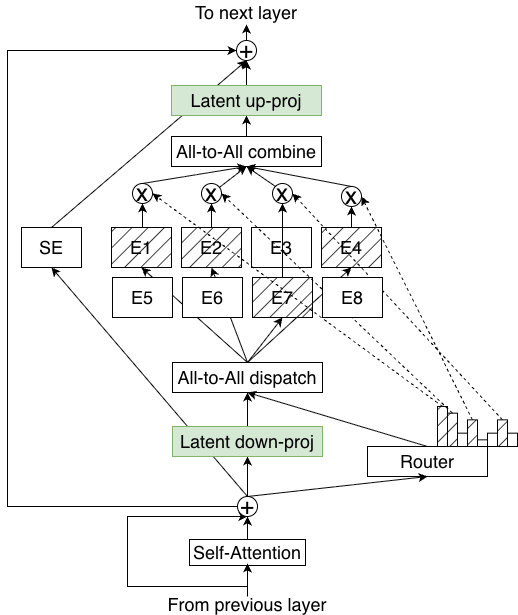
\includegraphics[width=\linewidth]{n3s-fig03b-latent-moe.png}
    \caption{LatentMoE}
  \end{subfigure}
  \caption[Standard MoE compared with LatentMoE]{Standard MoE compared with
  LatentMoE, where tokens are projected into a smaller latent dimension $\ell$
  for routing and expert computation. \source{NVIDIA
  (2026)~\cite{nvidia2026super}, Fig.~3}}
  \label{fig:latentmoe}
\end{figure}

In \NS, $d = 4096$ and $\ell = 1024$, so $\alpha = 4$. By the author's
estimate, the routed experts hold about 113 of the 120.6 billion parameters,
of which only $22/512 \approx 4.3\%$ are used per token---the reason the
active size is about a tenth of the total. On a 95B model with the same
setting, LatentMoE matched or improved on the baseline's validation loss
(Figure~\ref{fig:latentmoe-loss}).

\begin{figure}[!htbp]
  \centering
  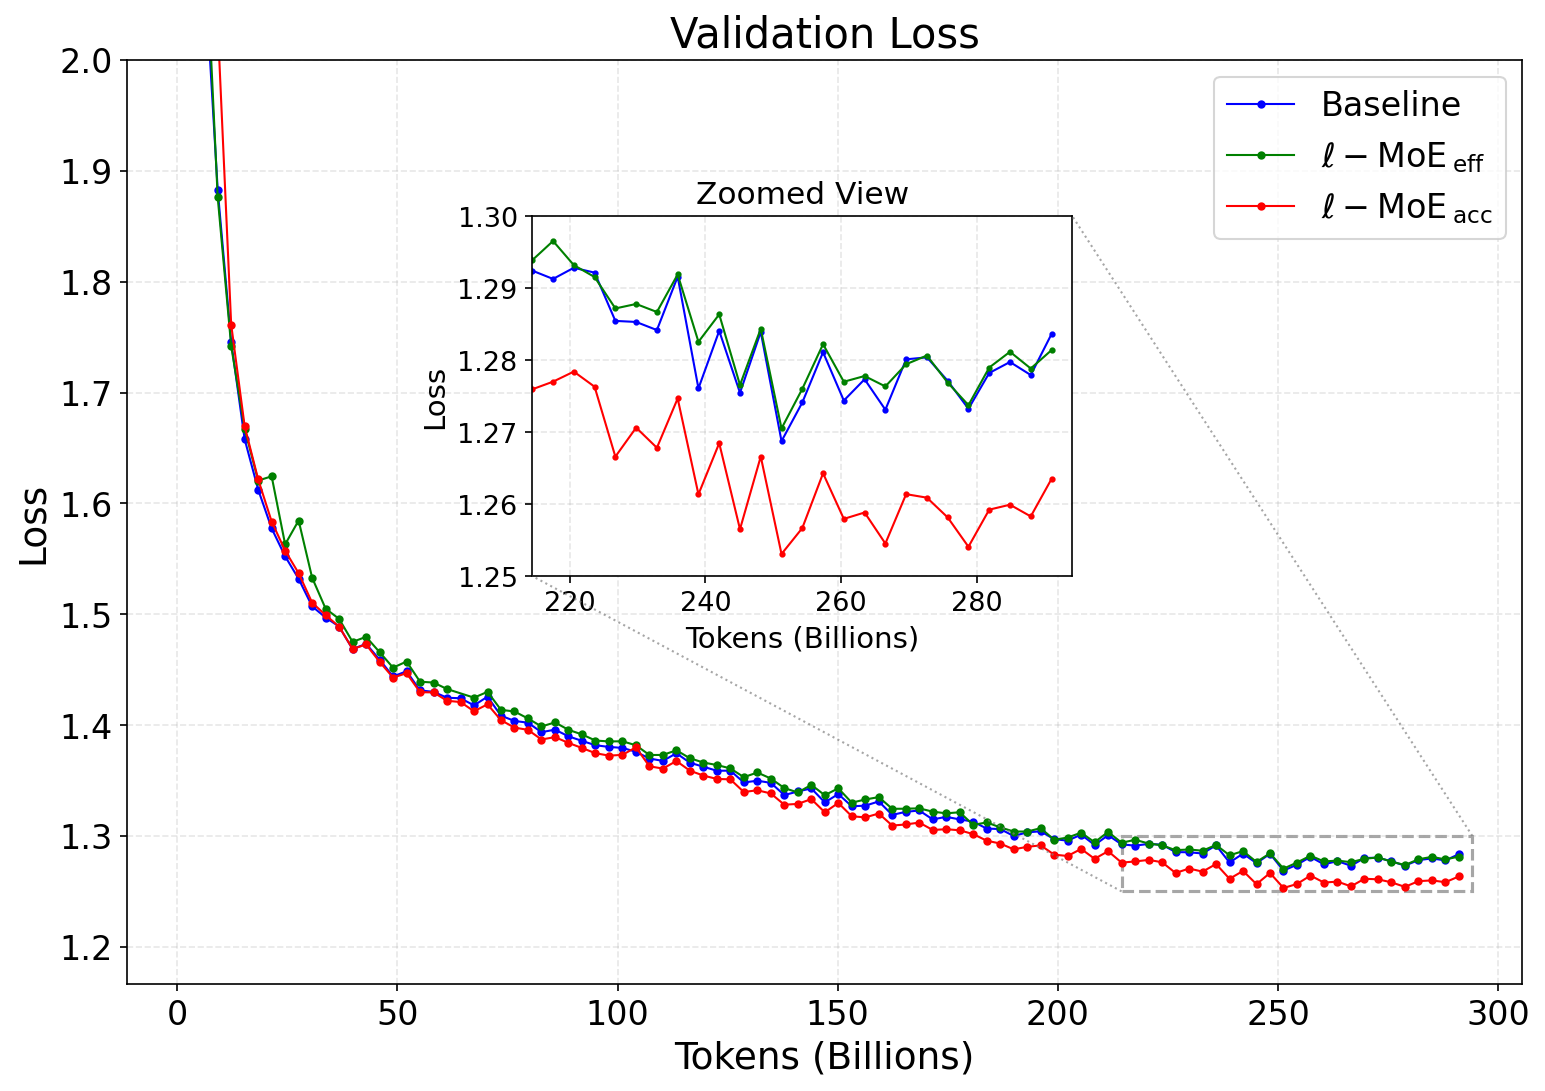
\includegraphics[width=0.6\linewidth]{latentmoe-fig06-95b-val-loss.png}
  \caption[Validation loss of LatentMoE variants on a 95B model]{Validation
  loss of a 95B baseline MoE and two LatentMoE configurations. \source{Elango
  et al.\ (2026)~\cite{elango2026latentmoe}, Fig.~6}}
  \label{fig:latentmoe-loss}
\end{figure}

\section{Multi-Token Prediction}

\NS\ adds an MTP objective~\cite{gloeckle2024mtp,deepseek2024v3}: auxiliary
heads also predict tokens further ahead, and the model is trained on
$\mathcal{L} = \mathcal{L}_{\text{next}} + 0.3\,\mathcal{L}_{\text{MTP}}$,
which improves validation loss and accuracy.

MTP also speeds up generation through speculative
decoding~\cite{leviathan2022speculative,chen2023speculative}: a cheap draft
proposes several tokens, the full model checks them in one pass, and the
agreeing ones are accepted (Figure~\ref{fig:specdec}). The output still
follows the full model's distribution. In \NS\ the MTP heads are the draft
model, so no separate network is needed and the extra computation is small.

Standard MTP uses independent heads, each trained for one fixed offset, which
limits a draft to as many tokens as there are heads. Reusing one head
repeatedly works poorly, because a head trained on ground-truth hidden states
is suddenly fed its own predictions. \NS\ instead \emph{shares the weights} of
its two MTP layers during training, giving a single head exposed to several
offsets. It is more robust to its own outputs, so it can be applied
recursively to draft longer sequences without adding parameters.

\begin{figure}[!htbp]
  \centering
  % Speculative decoding loop with MTP heads as the built-in draft model
\begin{tikzpicture}[
  font=\small, >={Stealth},
  stp/.style={rectangle, rounded corners=3pt, draw=gray!70!black, fill=blue!10,
              minimum height=1.35cm, text width=4.6cm, align=center}]
\node[stp] (ctx) at (0,0) {\textbf{1.} Current context\\$x_1,\dots,x_t$};
\node[stp, fill=green!18] (draft) at (7.2,0)
  {\textbf{2.} MTP head drafts $D$ tokens\\$\hat{x}_{t+1},\dots,\hat{x}_{t+D}$};
\node[stp, fill=orange!20] (verify) at (7.2,-2.6)
  {\textbf{3.} Main model verifies all $D$ drafts in \emph{one} forward pass};
\node[stp, fill=green!18] (keep) at (0,-2.6)
  {\textbf{4.} Keep the matching prefix ($a \le D$ tokens) plus the main model's own next token};
\draw[->, thick] (ctx) -- (draft);
\draw[->, thick] (draft) -- (verify);
\draw[->, thick] (verify) -- (keep);
\draw[->, thick] (keep) -- node[right, font=\footnotesize, align=left] {append $a+1$ tokens,\\repeat} (ctx);
\end{tikzpicture}

  \caption[Speculative decoding loop using MTP heads]{The speculative decoding
  loop, with the MTP head as the built-in draft model (drawn by the author).}
  \label{fig:specdec}
\end{figure}

On SPEED-Bench with a draft length of 7, \NS\ accepts on average 3.45 tokens
per verification step, more than DeepSeek-R1 (2.70) and Qwen3-Next (3.33), and
leads in eight of eleven categories (Table~\ref{tab:mtp}). Deeper drafts move
the throughput--latency curve outwards (Figure~\ref{fig:mtp-acceptance}).

\begin{table}[!htbp]
\centering
\small
\caption[MTP average acceptance lengths on SPEED-Bench]{MTP average acceptance
lengths on SPEED-Bench, draft length 7 (selected categories
from~\cite{nvidia2026super}, Table~2)}
\label{tab:mtp}
\begin{tabular}{@{}lccc@{}}
\toprule
\textbf{Category} & \textbf{DeepSeek-R1} & \textbf{Qwen3-Next} & \textbf{\NS} \\
\midrule
Coding        & 2.99 & \textbf{4.32} & 3.78 \\
Math          & 2.98 & \textbf{3.89} & 3.73 \\
Multilingual  & 2.83 & 3.97 & \textbf{4.05} \\
RAG           & 2.79 & 3.53 & \textbf{3.78} \\
Reasoning     & 2.80 & 3.47 & \textbf{3.59} \\
Summarization & 2.59 & 3.06 & \textbf{3.48} \\
\midrule
\textbf{Average (all 11)} & 2.70 & 3.33 & \textbf{3.45} \\
\bottomrule
\end{tabular}
\end{table}

\begin{figure}[!htbp]
  \centering
  \begin{subfigure}[b]{0.46\linewidth}
    \centering
    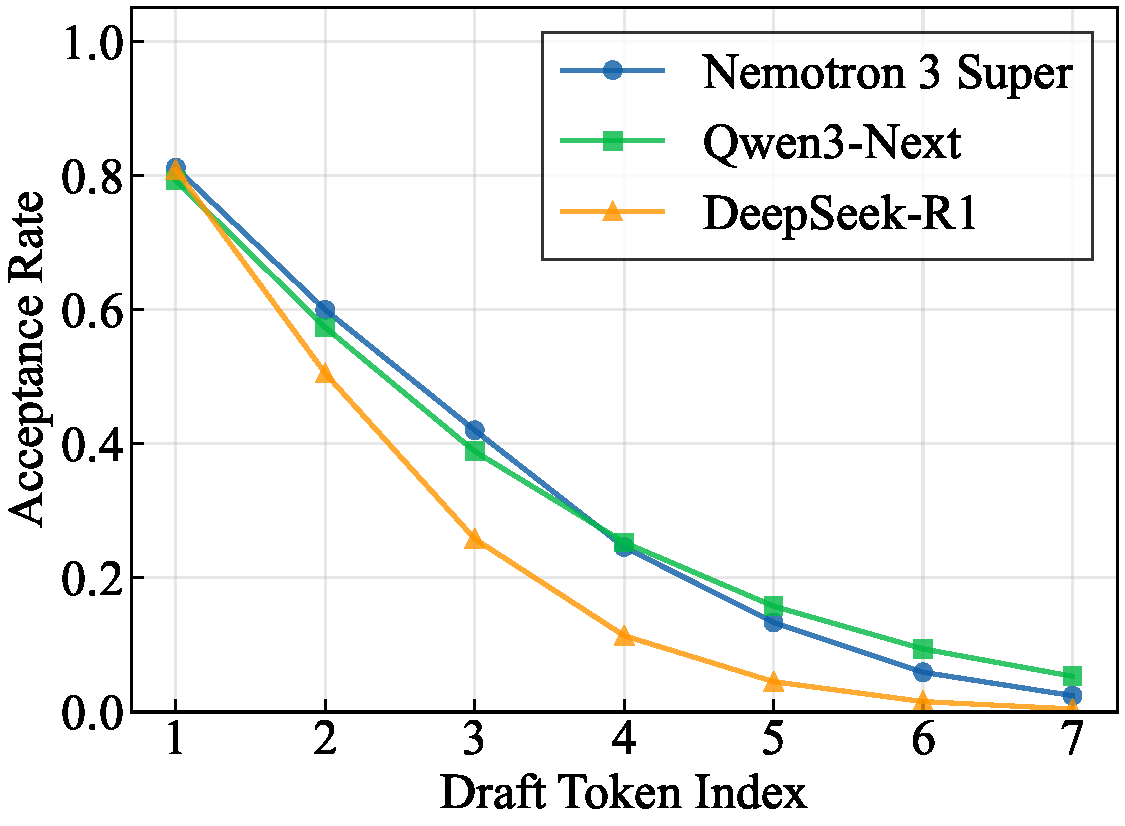
\includegraphics[width=\linewidth]{n3s-fig04-mtp-acceptance.pdf}
    \caption{Acceptance rate by draft index.}
  \end{subfigure}\hfill
  \begin{subfigure}[b]{0.44\linewidth}
    \centering
    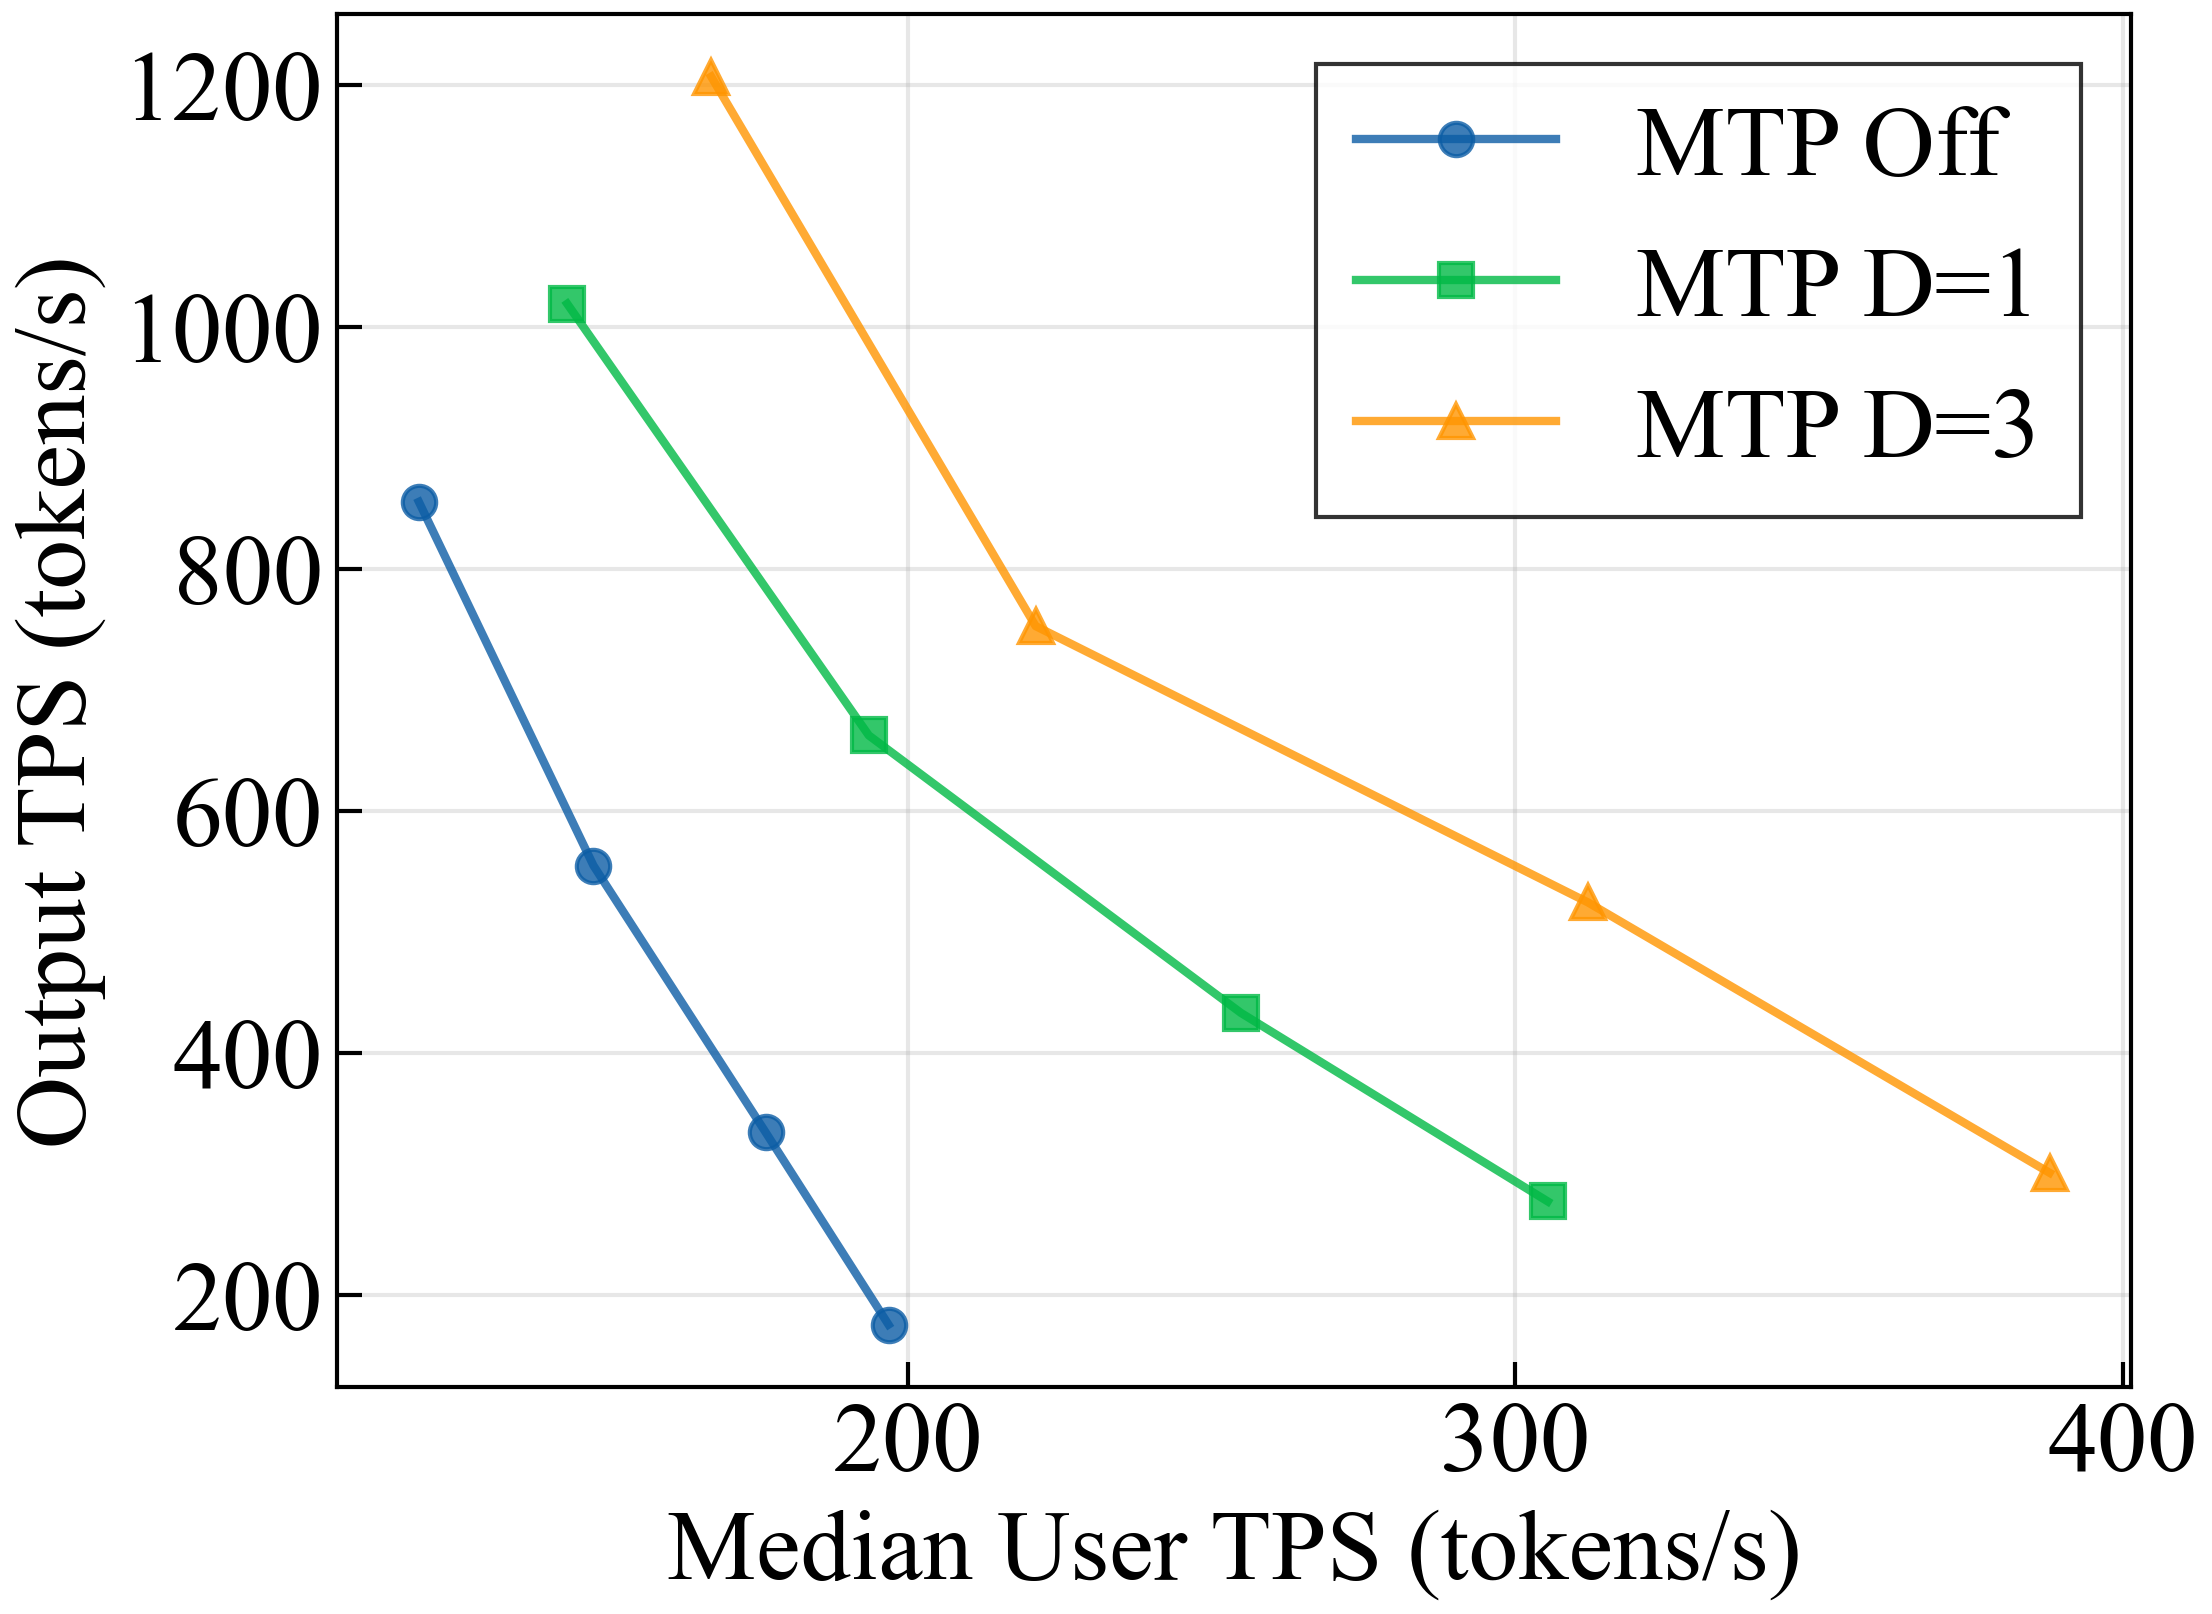
\includegraphics[width=\linewidth]{n3s-fig05-mtp-throughput.png}
    \caption{Throughput with MTP off and draft lengths 1 and 3.}
  \end{subfigure}
  \caption[MTP acceptance rate and serving throughput]{MTP acceptance on
  SPEED-Bench and its effect on serving throughput (NVFP4, B300 GPU).
  \source{NVIDIA (2026)~\cite{nvidia2026super}, Figs.~4 and~5}}
  \label{fig:mtp-acceptance}
\end{figure}

\section{Summary of the Architecture}

\NS\ arranges 88 layers so that 40 Mamba-2 blocks carry most of the sequence
processing, 8 GQA attention layers act as global anchors for exact retrieval,
and 40 LatentMoE layers provide capacity. LatentMoE compresses each token from
4096 to 1024 dimensions before routing, which cuts weight traffic and
communication fourfold and pays for 512 experts with 22 active per token. Two
shared-weight MTP layers improve training and act as a built-in draft model,
accepting on average 3.45 tokens per verification step. Together these choices
give a model with the capacity of 120 billion parameters, the per-token cost of
about 12 billion, and a KV cache only one sixth the size it would otherwise be.
